\section{Model and Design}
\label{sec:model}


A workflow is modeled as a directed acyclic graph (DAG), where each node in the DAG often represents a workflow task ($t$), and the edges represent dependencies between the tasks that constrain the order in which tasks are executed. Dependencies typically represent data-flow dependencies in the application, where the output files produced by one task are used as inputs of another task. Each task is a computational program and a set of parameters that need to be executed. 
%Figure~\ref{fig:model_odag} (left) shows an illustration of a DAG composed of four tasks. 
This model fits several workflow management systems such as Pegasus~\cite{Deelman:2005:PFM:1239649.1239653}, Askalon~\cite{Fahringer:2005:ATS:1064323.1064331}, Taverna~\cite{Oinn:2006:TLC:1148437.1148448} and {Galaxy~\cite{22559942}. }In this paper, we assume {that }there is only one execution site with multiple compute resources, such as virtual machines on the clouds. 


Figure~\ref{fig:model_system} shows a typical workflow execution environment. The {\textbf{submit host} }prepares a workflow for execution (clustering, mapping, etc.), and worker nodes, at an execution site, execute jobs individually. The main components are introduced below:

\begin{figure}[!htb]
\centering
  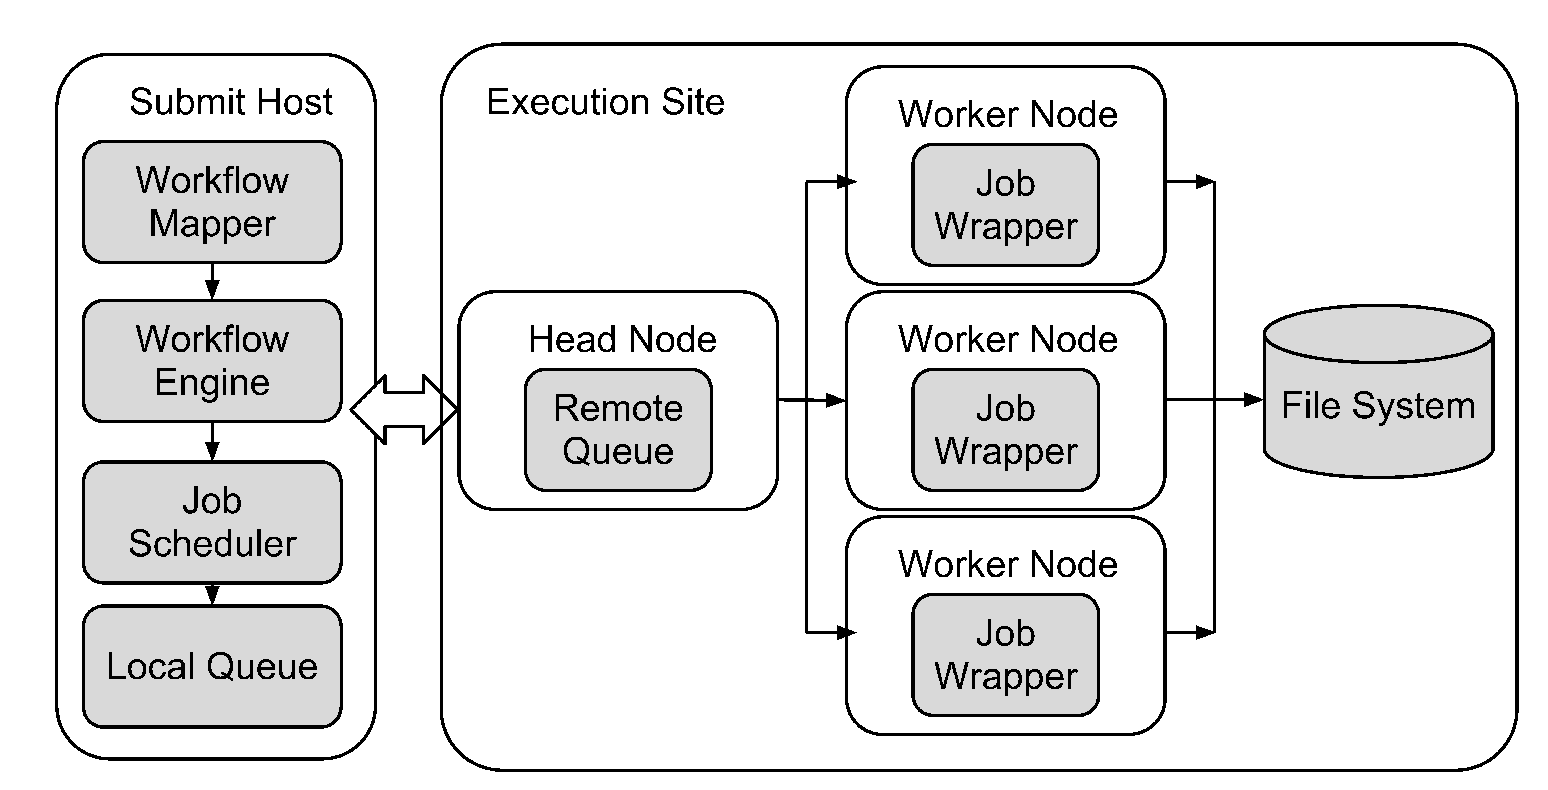
\includegraphics[width=0.95\linewidth]{figure1.eps}
  \caption{A workflow system model.}
  \label{fig:model_system}
\end{figure}

\paragraph{Workflow Mapper} Generates an executable workflow based on an abstract workflow~\cite{Deelman2004} provided by the user or workflow composition system. It also restructures the workflow to optimize performance and adds tasks for data management and provenance information generation. {The Workflow Mapper also merges }small tasks together into a job such that system overheads are reduced (\textbf{task clustering}). A job is a single execution unit in the workflow execution systems and is composed of one or more tasks. 


\paragraph{Workflow Engine} Executes jobs defined by the workflow in order of their dependencies. Only jobs that have all their parent jobs completed are submitted to the Job Scheduler. The elapsed time from when a job is released (all of its parents have completed successfully) to when it is submitted to the job scheduler is denoted as the workflow engine delay. %The workflow engine delay is usually configured by users to assure that the entire workflow scheduling and execution system is not overloaded. 

\paragraph{Job Scheduler and Local Queue} Manage individual workflow jobs and supervise their execution on local and remote resources. {The scheduler relies on the resources (compute, storage, and network) defined in the executable workflow to perform computations. }The elapsed time from when a task is submitted to the job scheduler to when it starts its execution in a worker node is denoted as the queue delay. It reflects both the efficiency of the job scheduler and resource availability. 

\paragraph{Job Wrapper} Extracts tasks from clustered jobs and executes them at the worker nodes. The clustering delay is the  elapsed time of the extraction process.

\begin{figure}[!htb]
	\centering
	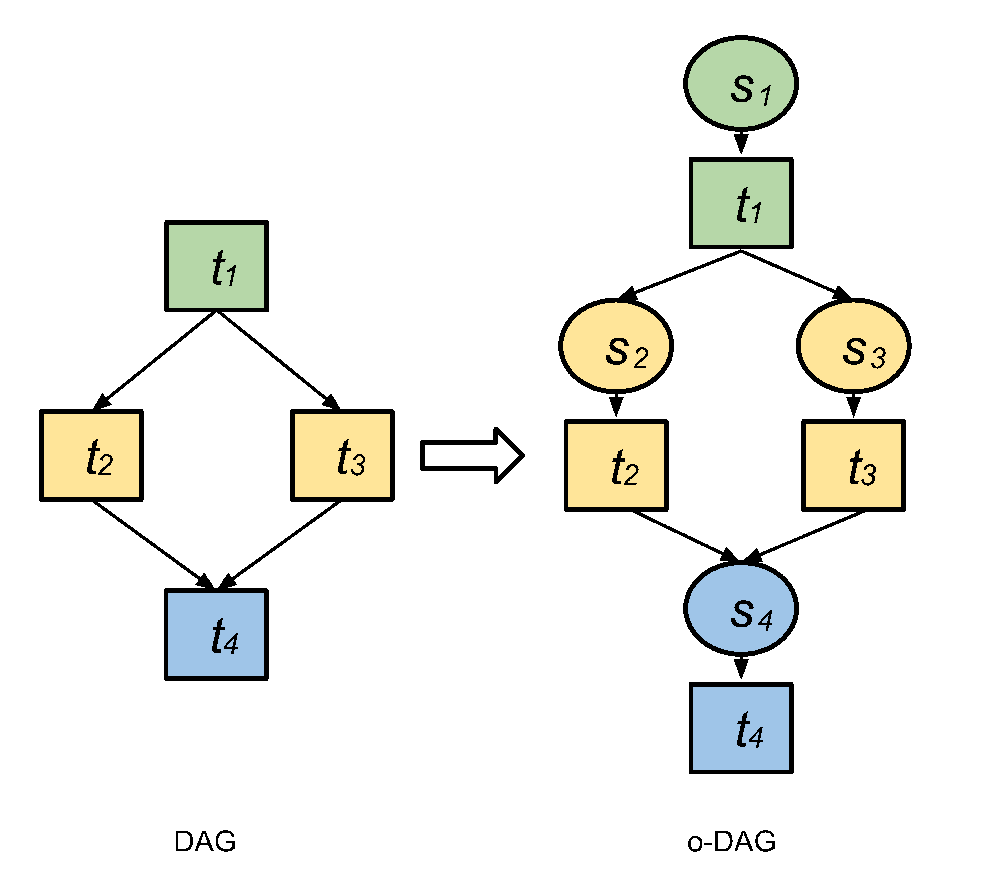
\includegraphics[width=0.7\linewidth]{figure2.eps}
	\captionof{figure}{Extending DAG to o-DAG (\emph{s} denotes a system overhead).}
	\label{fig:model_odag}
\end{figure}

We extend the DAG model to be overhead aware (o-DAG). System overheads play an important role in workflow execution and constitute a major part of the overall runtime when tasks are poorly clustered~\cite{Chen2011}. Figure~\ref{fig:model_odag} shows how we augment a DAG to be an o-DAG with the capability to represent system overheads ($s$) such as workflow engine and queue delays. In addition, system overheads also include data transfer {delays }caused by staging-in and staging-out data. This classification of system overheads is based on our prior study on workflow analysis~\cite{Chen2011}. 

With an o-DAG model, we can explicitly express the process of task clustering. In this paper, we address {horizontal and vertical task clustering}. \textbf{Horizontal Clustering} (HC) merges multiple tasks that are at the same horizontal level of the workflow, in which the horizontal level of a task is defined as the longest distance from the entry task{(s) }of the DAG to this task {(an entry task has no parents)}. \textbf{Vertical Clustering} (VC) merges tasks within a pipeline of the workflow. Tasks {in }the same pipeline share a single-parent-single-child relationship, which means a task $t_a$ is the unique parent of a task $t_b$, which is the unique child of $t_a$. 

Figure~\ref{fig:model_hc} shows a simple example of how to perform HC, in which two tasks $t_2$ and $t_3$, without a data dependency between them, are merged into a clustered job $j_1$. A job $j$ is a single execution unit composed by one or multiple task(s). Job wrappers are commonly used to execute clustered jobs, but they add an overhead denoted by the clustering delay $c$. The clustering delay measures the difference between the sum of the actual task runtimes and the job runtime seen by the job scheduler. 
After horizontal clustering, $t_2$ and $t_3$ in $j_1$ can be executed in sequence or in parallel, if parallelism {on }one compute node is supported. In this paper, we consider sequential executions only. Given a single resource, the overall runtime for the workflow in Figure~\ref{fig:model_hc} (left) is $runtime_l= \sum_{i=1}^{4}(s_i+t_i)$, and the overall runtime for the clustered workflow in Figure~\ref{fig:model_hc} (right) is $runtime_r=s_1+t_1+s_2+c_1+t_2+t_3+s_4+t_4$.  $runtime_l > runtime_r$ as long as $c_1 < s_3$, which is the case in many distributed systems since the clustering delay within a single execution node is usually shorter than the scheduling overhead across different execution nodes. 

\begin{figure}[!htb]
\centering
 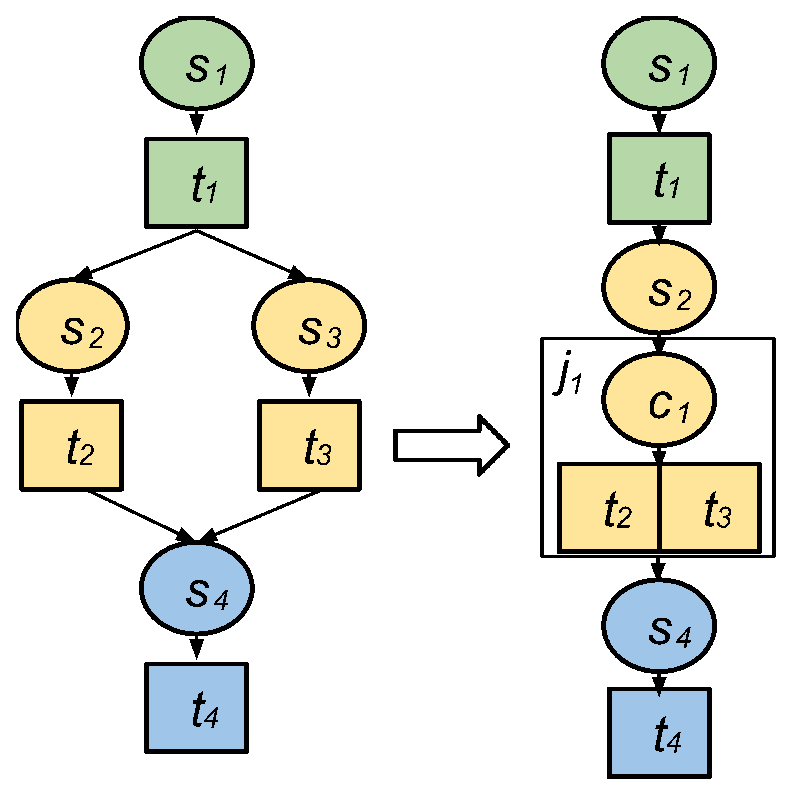
\includegraphics[width=0.5\linewidth]{figure3.eps}
  \captionof{figure}{An example of horizontal clustering (color indicates the horizontal level of a task).}
  \label{fig:model_hc}
\end{figure}

Figure~\ref{fig:model_vc} illustrates an example of vertical clustering, in which tasks $t_2$, $t_4$, and $t_6$ are merged into $j_1$, while tasks $t_3$, $t_5$, and $t_7$ are merged into $j_2$. Similarly, clustering delays $c_2$ and $c_3$ are added to $j_1$ and $j_2$ respectively, but system overheads $s_4$, $s_5$, $s_6$, and $s_7$ are removed. 




%Task clustering has been applied to many scenarios where resources are much less than tasks, which is true for many scientific workflows~\cite{Singh2008, Ying2009, Zomaya2004}, and has achieved significant improvement (i.e., 97\% as reported by ~\cite{Singh2008}) over the case without clustering. Table~\ref{tab:model_stats} shows the statistical workflow information (average task runtime etc. ) of six widely used scientific applications and their runtime information (number of nodes, average queue delay, etc.)~\cite{Chen2011}. For all of these workflows, there are a lot more tasks than available nodes and the average task runtime is shorted than system overheads. Therefore, task clustering can achieve significant improvement over no clustering. Besides the benefits of runtime improvement, task clustering also allows us to run on some federated distributed environment. For example, FutureGrid~\cite{FutureGrid} allows a user to use up to 20 VMs at a time. We will introduce the details of these workflows and distributed platforms in Session~\ref{sec:experiments}

%\begin{table*}[htbp]
%\centering
%\begin{tabular}{lrrrrrrrr}
%\hline
%Workflow & Venue & Nodes & Tasks & Workflow Engine Delay  &  Queue Delay  & Task Runtime  \\
%
%\hline
%
%SIPHT & UW Madison & 8 & 33 & 17 & 69 & 20\\ 
%Broadband & Amazon EC2 & 8 &770 & 17 &945&308\\
%Epigenomics &Amazon EC2&8& 83 &6&311&158\\
%CyberShake &Skynet&5&24142&12&188&5\\
%Montage &USC&20&10427&182&26136&523\\
%
%
%\hline
%\end{tabular}
%\caption{Overhead (in seconds) and Runtime Information }
%\label{tab:model_stats}
%\end{table*} 
